\documentclass[inputenc=utf8]{ldvarticle}

    
% Packages
\usepackage{float}
\usepackage{natbib}
\bibliographystyle{plain}
\usepackage{hyperref}
\usepackage{graphicx, import}   % Pictures
\usepackage{lipsum}             % Blindtext
\usepackage[usenames,dvipsnames]{xcolor}
\usepackage{fancyhdr}

\def\code#1{\texttt{#1}}

\begin{document}
%---------------------------------------------------------------------------------------
\begin{titlepage}

%%% Logo
	\noindent
	\begin{tabular}[t]{@{}l} 
  	
\includegraphics [scale= 0.4]{./img/Logo/LDVLogoS_oT.pdf}\\[0.2cm]
	\end{tabular}
	\hfill% move it to the right
	\begin{tabular}[t]{l@{}}
	
\includegraphics[scale= 0.8]{./img/Logo/TUMLogo_oZ_Vollfl_sw.pdf}\\[0.2cm]	
	\end{tabular}
%%% End Logo
	
\begin{center}

	\vspace{\stretch{0.7}}
	\Huge \textbf {Engineering Practice Report} \\
	\vspace{\stretch{0.02}}
	\huge{Deep Motion Planning for Autonomous Driving}\\
	\vspace{\stretch{0.15}}
	\Large{August 16, 2021 - November 12, 2021 }
	%\vspace{\stretch{0.6}}\noindent
	
	\vfill\noindent
	% Tabellen Beispiel
	\begin{table}[h!]
	\centering
	\begin{tabular}{ll}
	\textbf {Student}& Pei-Yi Lin       \\
	student ID number & 03728797                   \\
	  & \underline{peiyi.lin@tum.de} \\
	\\
	\textbf {Supervisor}  & Stefan Matthes          \\
	 & fortiss GmbH                           \\
	& Guerickestraße 25,                          \\
	& 80805 München                          
	\end{tabular}
	\end{table}

		
	%\end{center}
\end{center}
\end{titlepage}

% =====================================
\pagebreak[4]

%\maketitle
% Chapters
%\section*{Abstract}
\addcontentsline{toc}{chapter}{Abstract}
\lipsum[4]

\section*{Abstract}
In the 3-month internship, I had the chance to take a detailed look how deep learning algorithms can be applied to autonomous driving, especially in the part of motion planning. I started with literature review, and later on reimplemented a repository from a previous research, Learning by Cheating \cite{chen2019lbc}. \\
\noindent \\I have put my code on GitHub. \url{https://github.com/b07901064/public_1}

% Section 1 ========================
\section{Motivation and Goal of the Project}
I am deeply interested in the field of machine learning. I’ve already taken courses in university. However, I didn’t have many opportunities to put the theory into practice. Therefore, I am motivated in an internship that would somehow relate to machine learning. Luckily, I got the chance to work on the Carla autonomous driving project in fortiss \cite{Dosovitskiy2017CARLAAO} \footnote {\url{https://www.kiwissen.de}} \footnote {\url{https://www.fortiss.org/forschung/projekte/detail/ki-wissen}}.
\\

\noindent Machine learning algorithms has several applications, and autonomous driving is one of them. It is also a widely discussed topic in recent years. I am really found of the topic, and I was excited that I might have the opportunity to learn how deep learning algorithms can be applied to autonomous driving. Originally, my goal was to first read about some of the state-of-the-art approaches, and then implement an algorithm for motion planning.

% Section 2 ========================
\section{Technical Background and Starting Point for the Work}

I am currently in my 5th bachelor semester studying electrical and computer engineering. Before the internship, I had only two courses concerning machine learning, which were “Machinelle Intelligenz und Gesellschaft” and “Introduction to Machine Learning”. Through these courses, I’ve learnt some theories and traditional machine learning algorithms, e.g. regression, SVM, decision tree, clustering, and I had practiced some programming exercises. To be honest, I never have had a course that focuses on simply teaching Python, the programming language. Thus, even though I knew Python, I did not really have a solid foundation in it.
\\

\noindent In addition, I didn’t know much about deep learning. It was only briefly introduced in the university lecture. Moreover, neither did I hold experiences in PyTorch nor Tensorflow.
\\

\noindent Hence, I started with literature review on state-of-the-art deep learning-based approaches (see the References). Most of the paper I read used either imitation learning or reinforcement learning. Yet, I was not familiar with neither the two machine learning areas, but I’ve learnt a lot during the process. After reading the articles, I felt that I’d personally prefer the imitation learning approach. There was one paper I particularly liked , which is Learning by Cheating \cite{chen2019lbc}. Therefore, I decided to implement an algorithm based on their approach.
\\

\noindent After two weeks of literature review, I spent another week at home looking into the syntax of the framework, PyTorch, before I started to set up the working environment in the office. My colleges introduced the cloud computing concept to me, i.e. how I can connect to their server and work in my docker container. I also learnt to use conda environment to manage dependencies and isolate projects. At the same time, since I was working on an Ubuntu machine, I got more familiar with the terminal as well.
\\

\noindent During the internship, I tried out two repositories. The first repository requires users to collect data with the Carla server. Since installing a Carla simulator on the company server is not an easy task, the plan was originally first collect data on the local machine with the installed Carla server, and then upload the collected data to the company server and train the model there. I’ve install multiple versions of Carla simulator. For each simulator, I had to set up a virtual environment, and specified the correct \code{\$PYTHONPATH} and sometimes custom .egg files. The authors loaded the data in a complicated format which we couldn’t really use. Therefore, with the help of my supervisor, I wrote a data loader file to load data in binary format with the module pickle. It is an easy and efficient way to load data. I was able to load the data and see channels of images. However, when I went back after the weekend, it seemed that I could not establish connection between the client and Carla server, even though I didn’t change anything. At the end, we gave up on that repository because we had seen too many problems with it. For instance, the provided environment was really out dated, that was why we had to try different versions of Carla simulator and spend quite some time just to set up the environment.
\\

\noindent The second repository is from the same author. It’s from his another paper \cite{Chen2021LearningTD} about their reinforcement learning approach to the Carla autonomous driving challenge, but he also included their LBC code in the repository. The environment provided in the second repository is more up-to-date and it doesn’t contain many other unnecessary packages. They also provide a dataset online, so that I didn’t really have to collect data with the Carla server myself. I downloaded the dataset and basically start my real work from there.

% Section 3 ========================
\section{Solution Concept and Realization of the Project}

% 3.1 ========================
\subsection{Data Loader}
My task then was to implement a baseline. At first I had no idea where to start, I stared at their code for days and there were a lot of thing I couldn’t understand. To solve this issue, I asked a college for some instructions, he suggested that I should start from loading the data.
\\

\noindent The provided dataset is in another format than the one the author used. The authors had the data in lmdb format, whereas the one I downloaded contains many subfolders, and each subfolder includes one folder with the images and a .json file which contains the numerical values and images file path. The whole dataset is hundreds GB large. I had to write a data loader to load the data efficiently, in terms of both memory and speed.
\\

\noindent I first had to define what information one item contains. One item could be the whole scenario, i.e. the whole subfolder, or it could also just be the information from one timeframe. We looked into their code, and we guessed they used just the information from one timeframe plus some future ego-vehicle’s locations for each item.
\\

\noindent I had some futile attempts at first. I was copying the data from one list to another, which is very inefficient. And then I figured out a way to access the data correctly. I then loaded the data from each subfolder as a SingleDataset and then I put these SingleDatasets in a list, and later concatenate all the SingleDataset into one big ConcatDataset. I can adjust how many data I’d want to load, and also how many future ego-vehicle’s locations I’d like to include for each item, however I like. Most of the time I only wanted to debug and see if the code works, so I could just load a small dataset, and it won’t take too long for me to test. If I wanted to train the model seriously, I could also load more data.
\\

\noindent After I finished loading the data. I could finally start building the network.


% 3.2 ========================
\subsection {BEV Model}
The birds-eye-view model (BEV model), is the privileged model. It has the BEV map as input, and it outputs the predicted locations for some future time frames (it can also be specified). The authors used ResNet-18 as backbone, added a speed encoder, and fed the output from the ResNet and speed encoder to a 3-layer convolutional network, and then they applied a Softmax layer to produce a spatial probability distribution, so basically a heat map of predicted locations for each future timeframe and for each command.
\\

\noindent The BEV model is relatively easy to train. I could use batch size of 256 on one GPU. And the model learns fast. The loss decreases drastically in the first episode, and continues to decrease in the later episodes. The output trajectory speaks to the ground truth trajectory after one episode, and it should also be a drivable trajectory.
%[]
\begin{figure}[H]
  \centering
  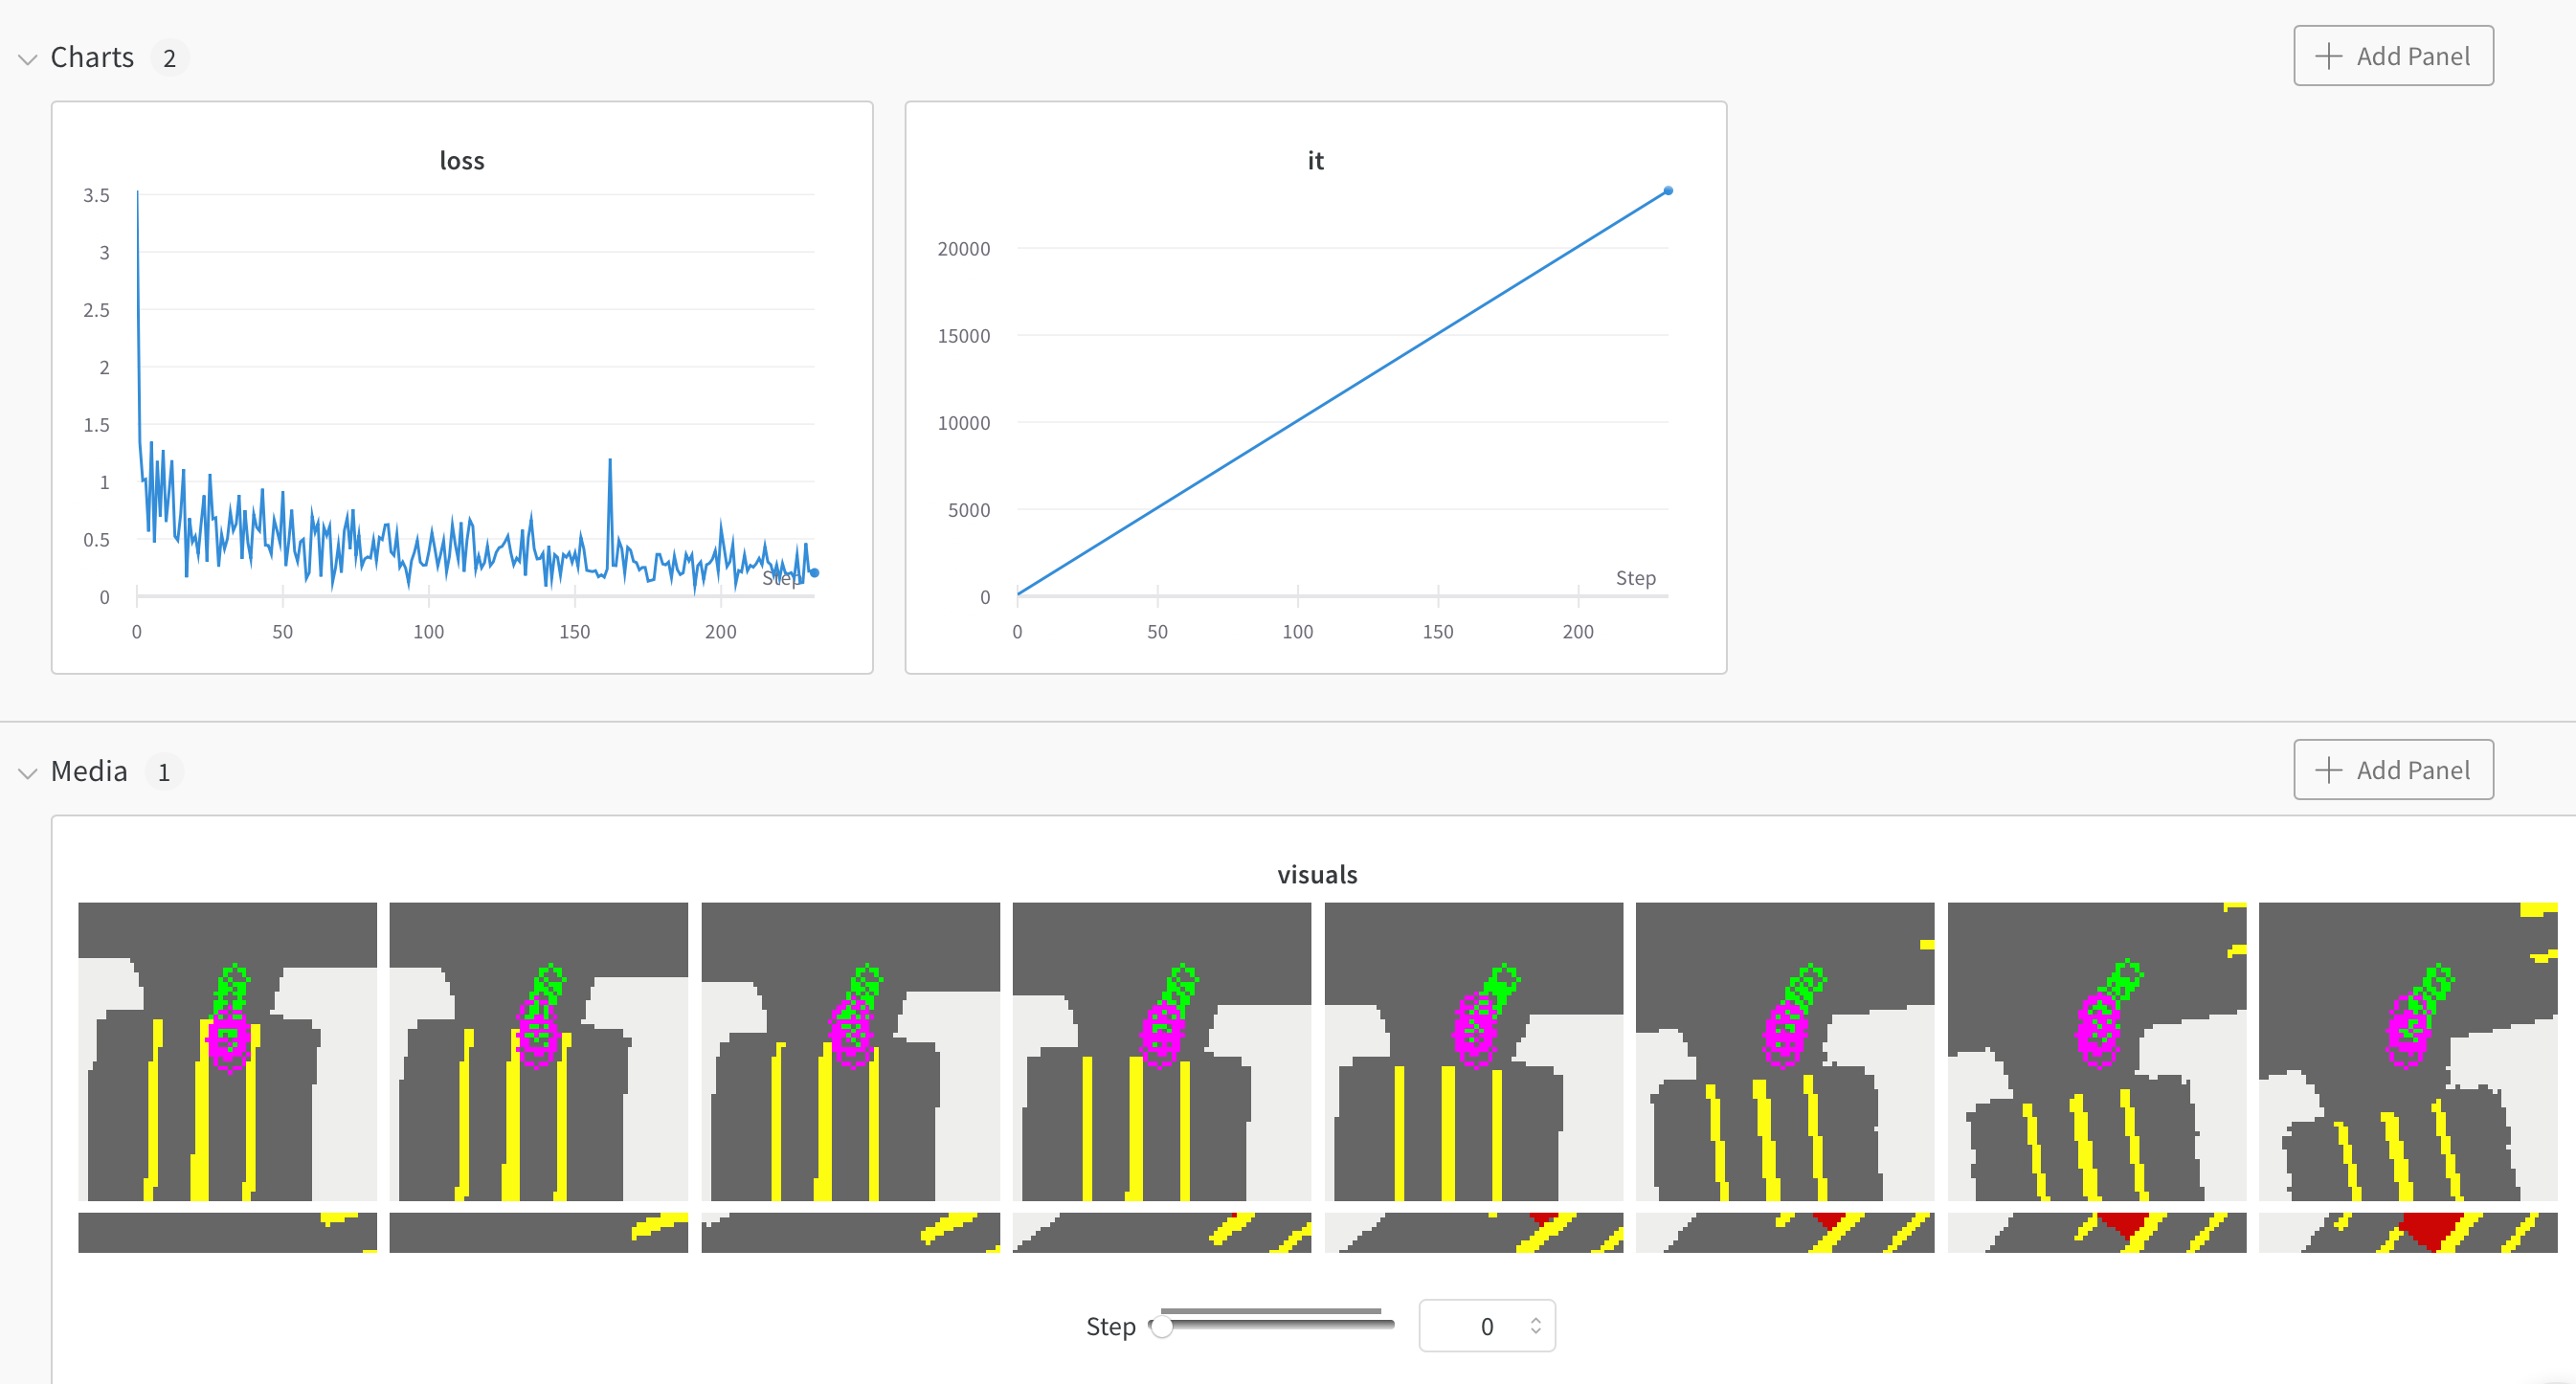
\includegraphics[width=0.8\textwidth] {bilder/cool_microwave_1.png} %[scale=1]{bilder/example_signal} % oder statt scale auch [width=0.5\textwidth] für eine feste Größe
  \caption{(green: ground truth, pink: predicted trajectory.)The model did not know how to drive at first and stayed where it was.}
  %\label{fig:somesignal}
\end{figure}

\begin{figure}[H]
  \centering
  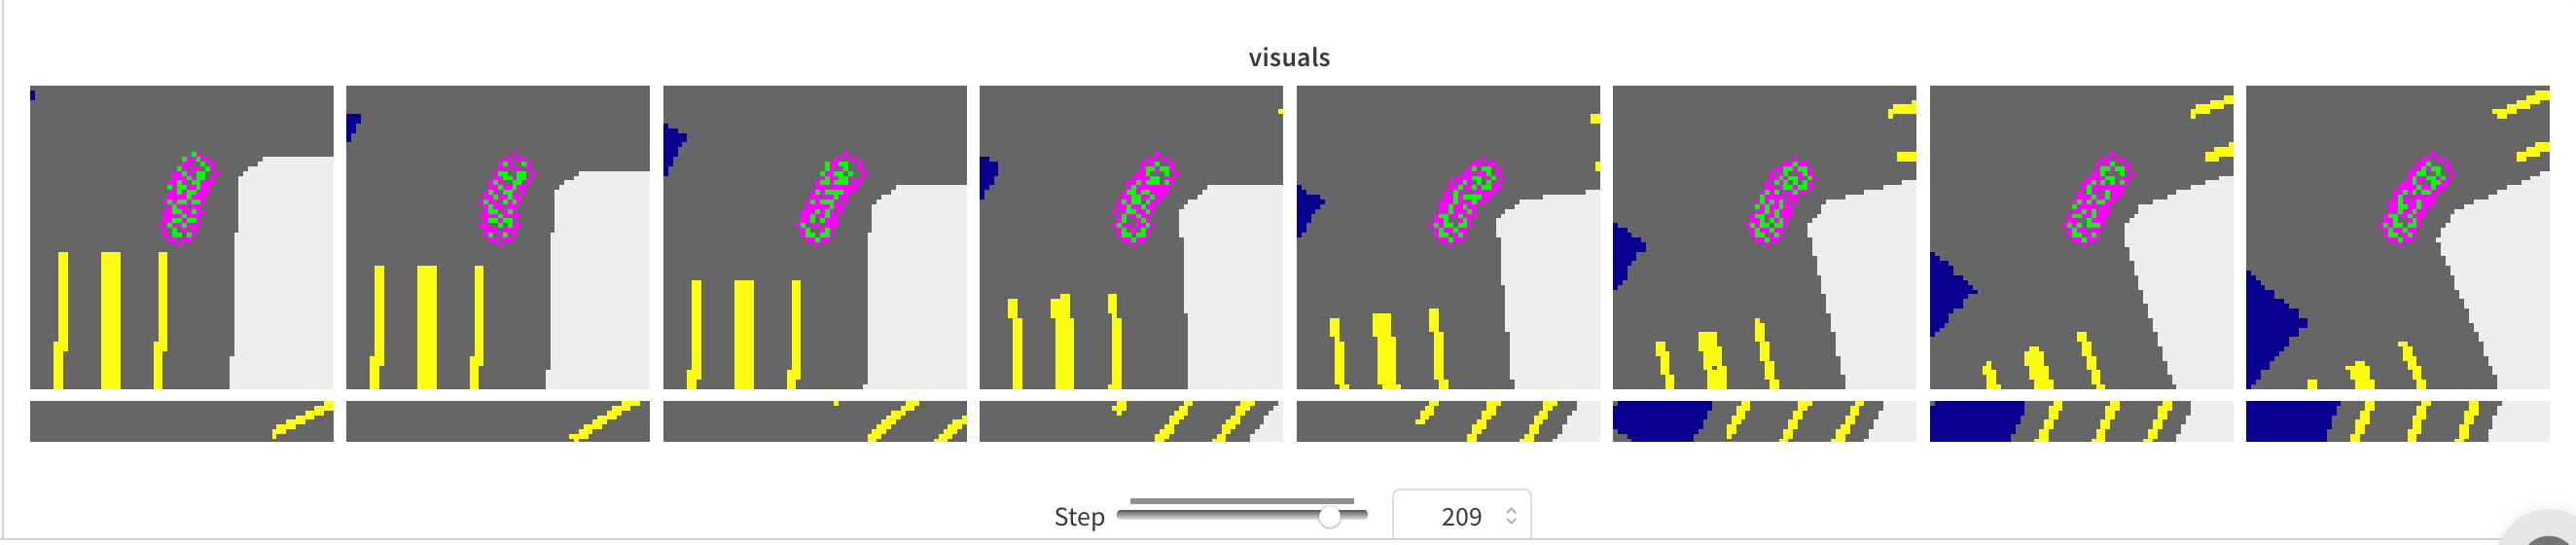
\includegraphics[width=0.8\textwidth] {bilder/cool_microwave_2.png} 
  \caption{(green: ground truth, pink: predicted trajectory.) After some training, the predicted trajectory is very close to the ground truth trajectory. }
 % \label{fig:somesignal}
\end{figure}


% 3.3 ========================
\subsection{RGB Model}
The camera-view model (RGB model). Takes extra two inputs, i.e. the RGB images from the frontal camera plus the segmented images. This model uses the output trajectory from the BEV model as the ground truth (tgt\_bev\_locs). 
\\

\noindent The RGB model network then takes only the RGB images and speeds (rgbs, spds) as input, and outputs the predicted locations on the RGB images (pred\_rgb\_locs), and also the predicted segmentations (pred\_sems). The predicted locations on the RGB images are then mapped to the birds-eye-view image (pred\_bev\_locs). We can calculate the loss between the predicted location and the ground truth; this loss is called act\_loss. In this case, the L1-loss is used. And act\_loss has 6 columns, where each column corresponds to a command. The location loss (loc\_loss) is calculated from the act\_loss, dependent on if the command is to follow a lane or to turn. Meanwhile, the model also tries to learn the segmentation. Namely, how to perceive and understand the RGB images from the frontal cameras.

\noindent \\The segmentation did not work at first. The model should label the RGB images. However, I did not provide the right ground truth segmentation for it to learn. Since it is all about labelling the images, the ground truth segmentation should be just labels, and has the size of (height, width, num\_labels). I didn’t know about that at first. From what I saw in the dataset, the segmented images are only .png files. I was not aware that my dataset is different from the one the authors used. If I read it as normal images, it would then have the wrong dimension in the 3rd order, so I just read it as gray-scale images. This way the ground truth values are just zeros. As a result, when I visualize the training process, the ground truth segmentation was all black, and the model learnt the segmentation to be all black, too. Nonetheless, even without the segmentation, the RGB model can still learn pretty well.
\\

\noindent The RGB model is more difficult to train. It takes more inputs, uses a bigger model, and it also requires the previously learnt BEV model. Thus, it also takes more GPU memory. I could only use batch size of 56 in this case. Ideally, I’d like to use a batch size of 128 or above. In the beginning, I didn’t pass the learnt BEV model, and the output did not make much sense. Both ground truth locations and predicted locations looked like random points and the trajectories were definitely not drivable.
%[figure]
\\

\noindent After I passed the BEV model, the trajectories started to make some sense. I could see the reasonable ground truth trajectory from the very beginning. The predicted trajectory, on the other hand, took a while to make sense. It first learnt how fast it should drive, and stopped when it needed to stop. For instance, it should stop at red light. However, I could not see the model turning before I went to bed. To my surprise, when I woke up the next morning and check again, I was thrilled to see the model slowly learning how to turn left and right. 
%[figure]
\\

\noindent There is one scenario that was captured by the logger more than once. From the two figures, we can observe that the model didn’t know how to turn at first, and in the later episode, it learnt to turn better, and produced a predicted trajectory closer to the ground truth.
% laced_thunder ...........................................................................
\begin{figure}[H]
  \centering
  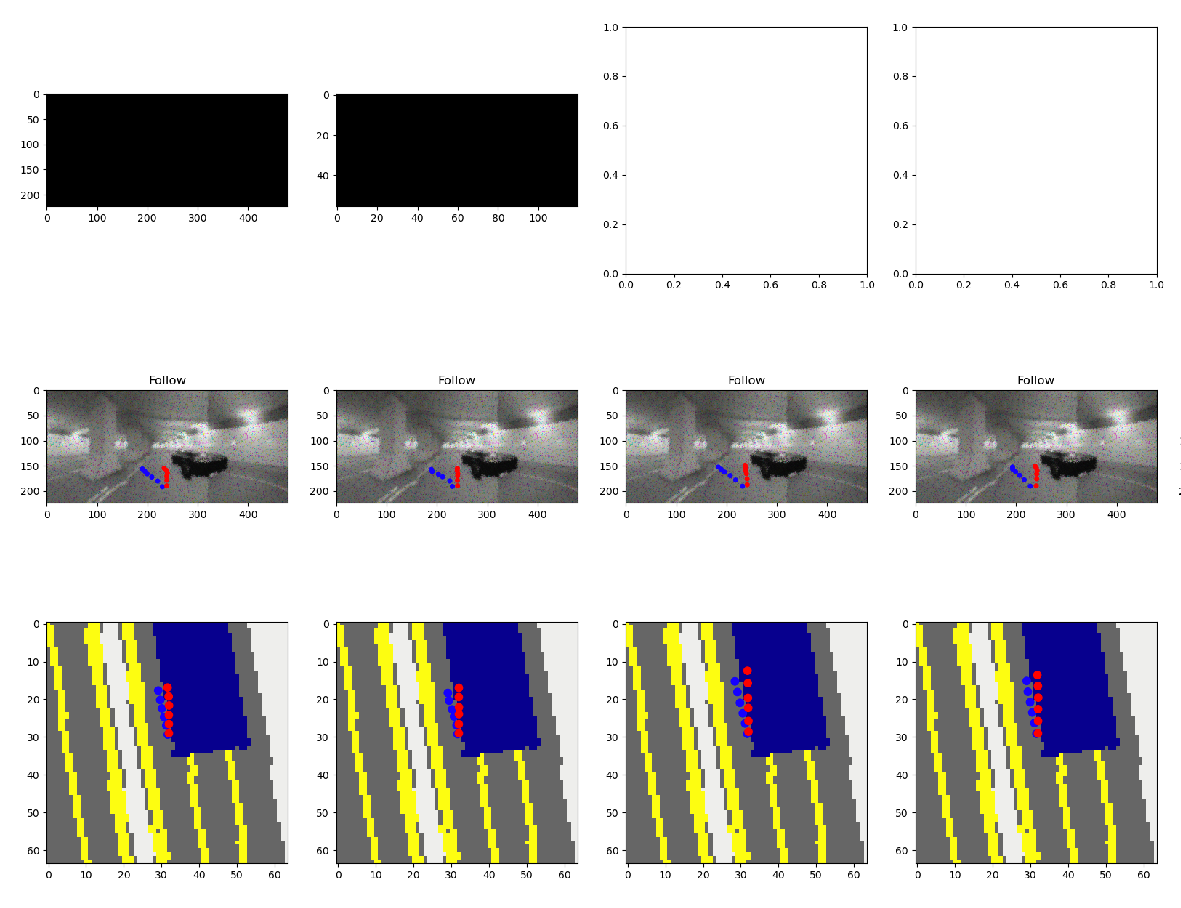
\includegraphics[width=0.75\textwidth] {bilder/lace_thunder_27.png} 
  \caption{(blue: ground truth, red: predicted trajectory.) The model only knew to drive straight. }
  %\label{fig:somesignal}
\end{figure}

\begin{figure}[H]
  \centering
  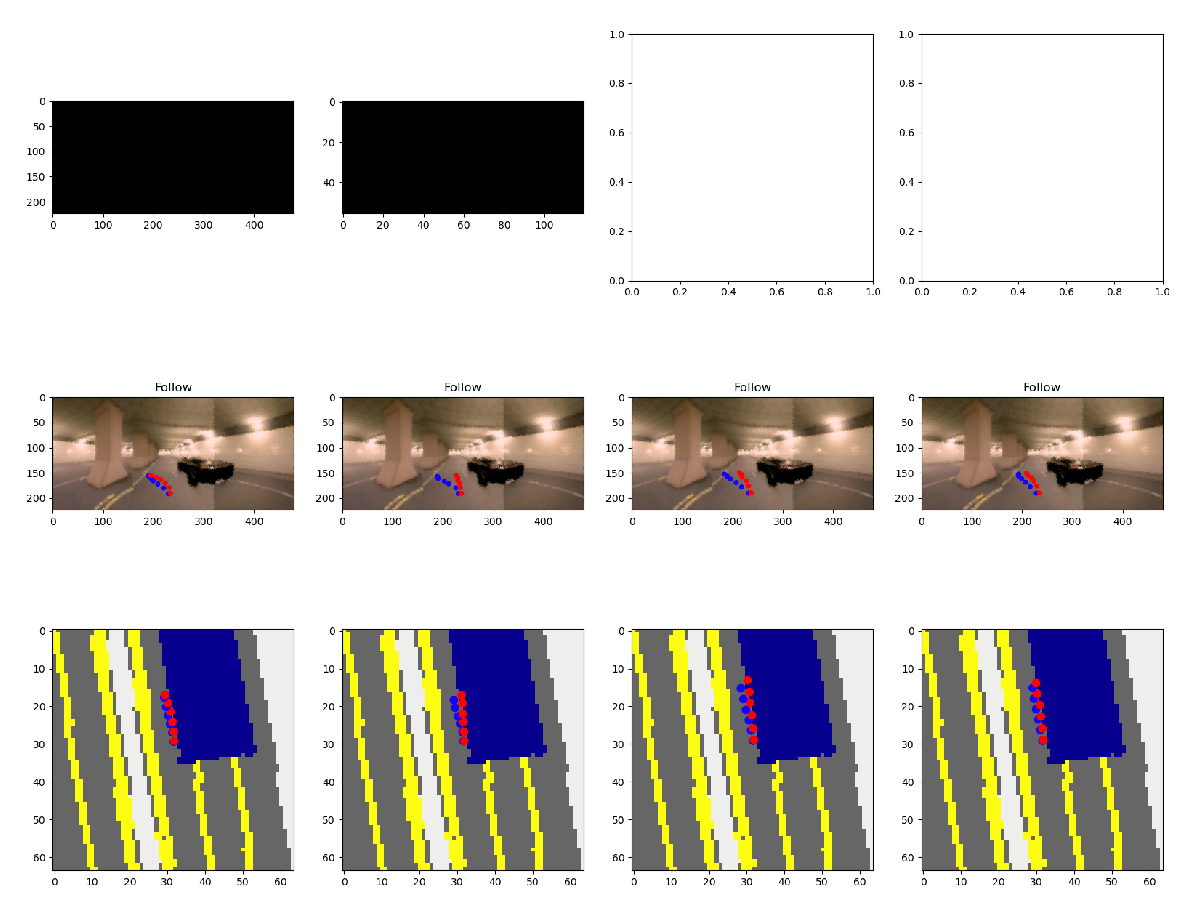
\includegraphics[width=0.75\textwidth] {bilder/lace_thunder_120.png} 
  \caption{(blue: ground truth, red: predicted trajectory.) Later on, the model has learnt how to turn better.}
  %\label{fig:somesignal}
\end{figure}

% laced_thunder ...........................................................................

\noindent \\Later on, I wanted to get my model to learn the segmentation as well. I fixed my dataloader. This way, I can first map the RGB values to labels and have the right segmentation as the ground truth. The cross entropy loss will then be computed between the ground truth and the predicted segmentation. The cross entropy loss function provided in PyTorch (torch.nn.functional.cross\_entropy) only takes the data of type “long” as input. That was a point we wanted to optimize. Since we were tight on GPU memory, we tried to write a custom function to calculate the cross entropy. After all, the cross entropy formula is not that complicated, and the segmentations are just labels that could be stored in a byte. However, we had to call torch.gather(), and it only take the data of type “long” as input. Unfortunately, it turned out that it was not something we could optimize on.
\\
\noindent \\Up to now, I have got the model to learn how to recognize the road, but it has not yet learnt how to recognize other objects.
\vspace{\stretch{0.04}}
% northern pyramid ..................................................
\begin{figure}[H]
  \centering
  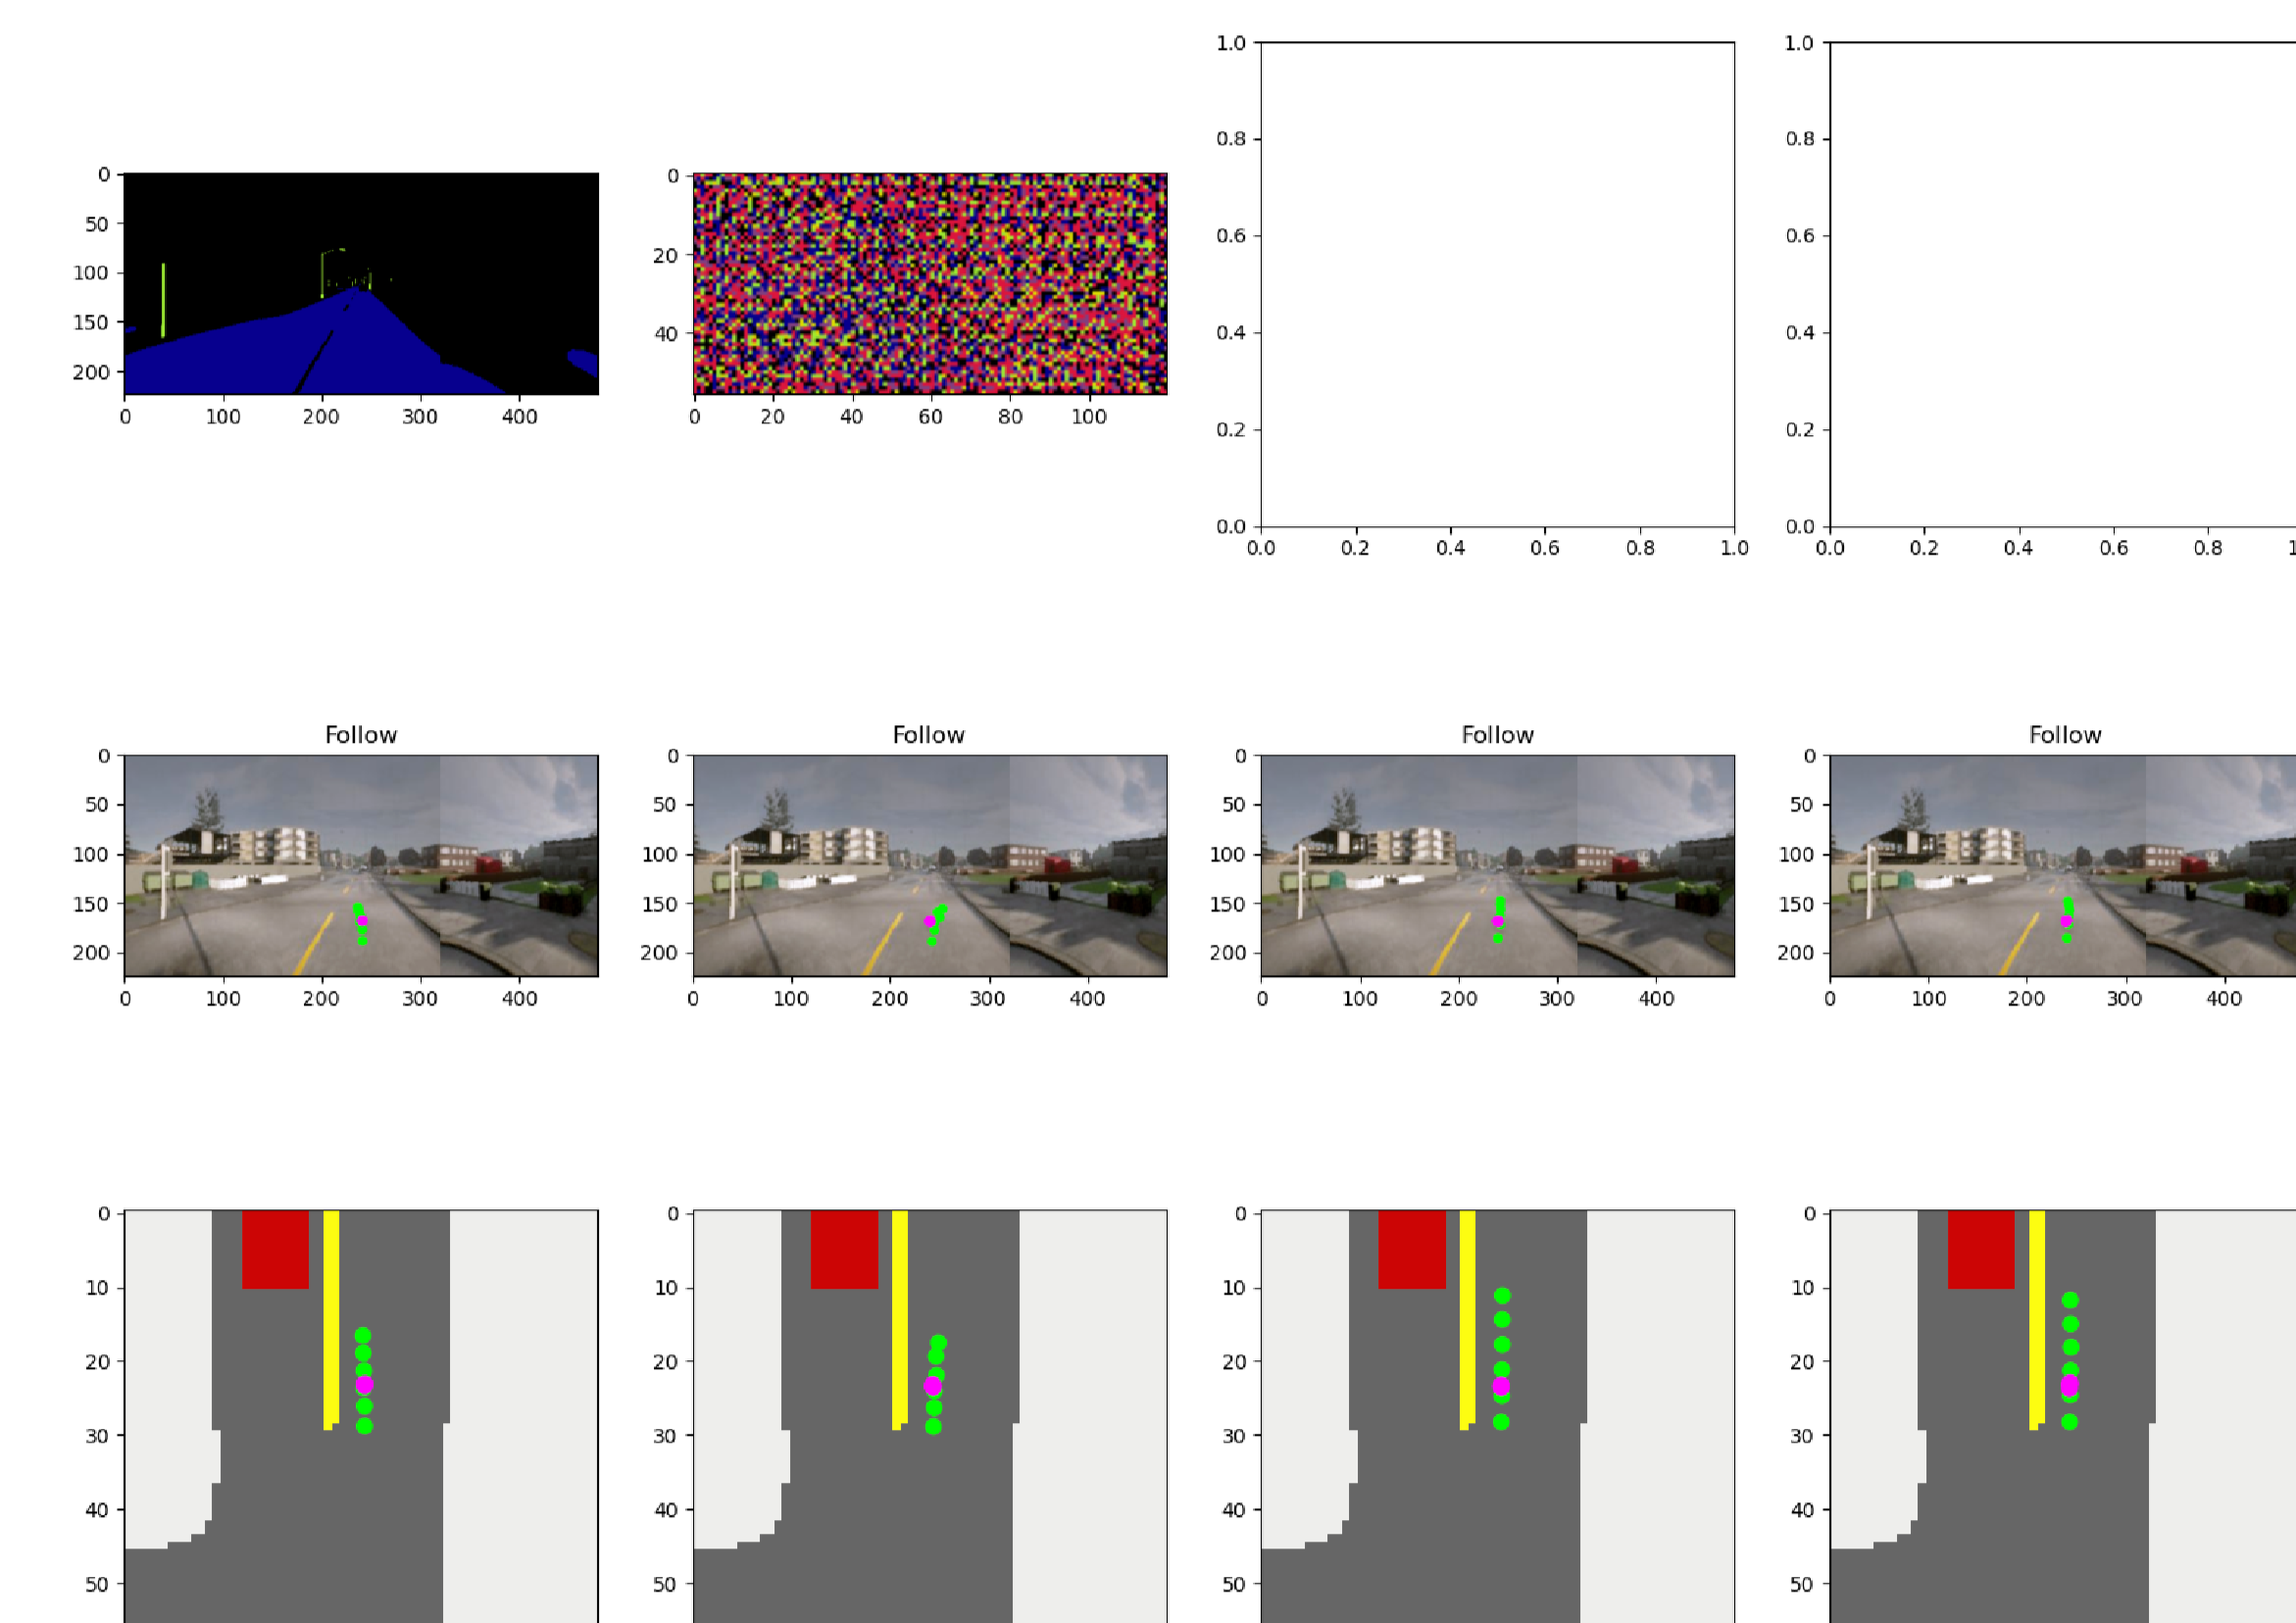
\includegraphics[width=0.8\textwidth] {bilder/northern_pyramid_0.png} 
  \caption{(green: ground truth, pink: predicted trajectory.) The model has not yet learnt how to drive, nor how to perceive the images.}
  %\label{fig:somesignal}
\end{figure}

\begin{figure}[H]
  \centering
  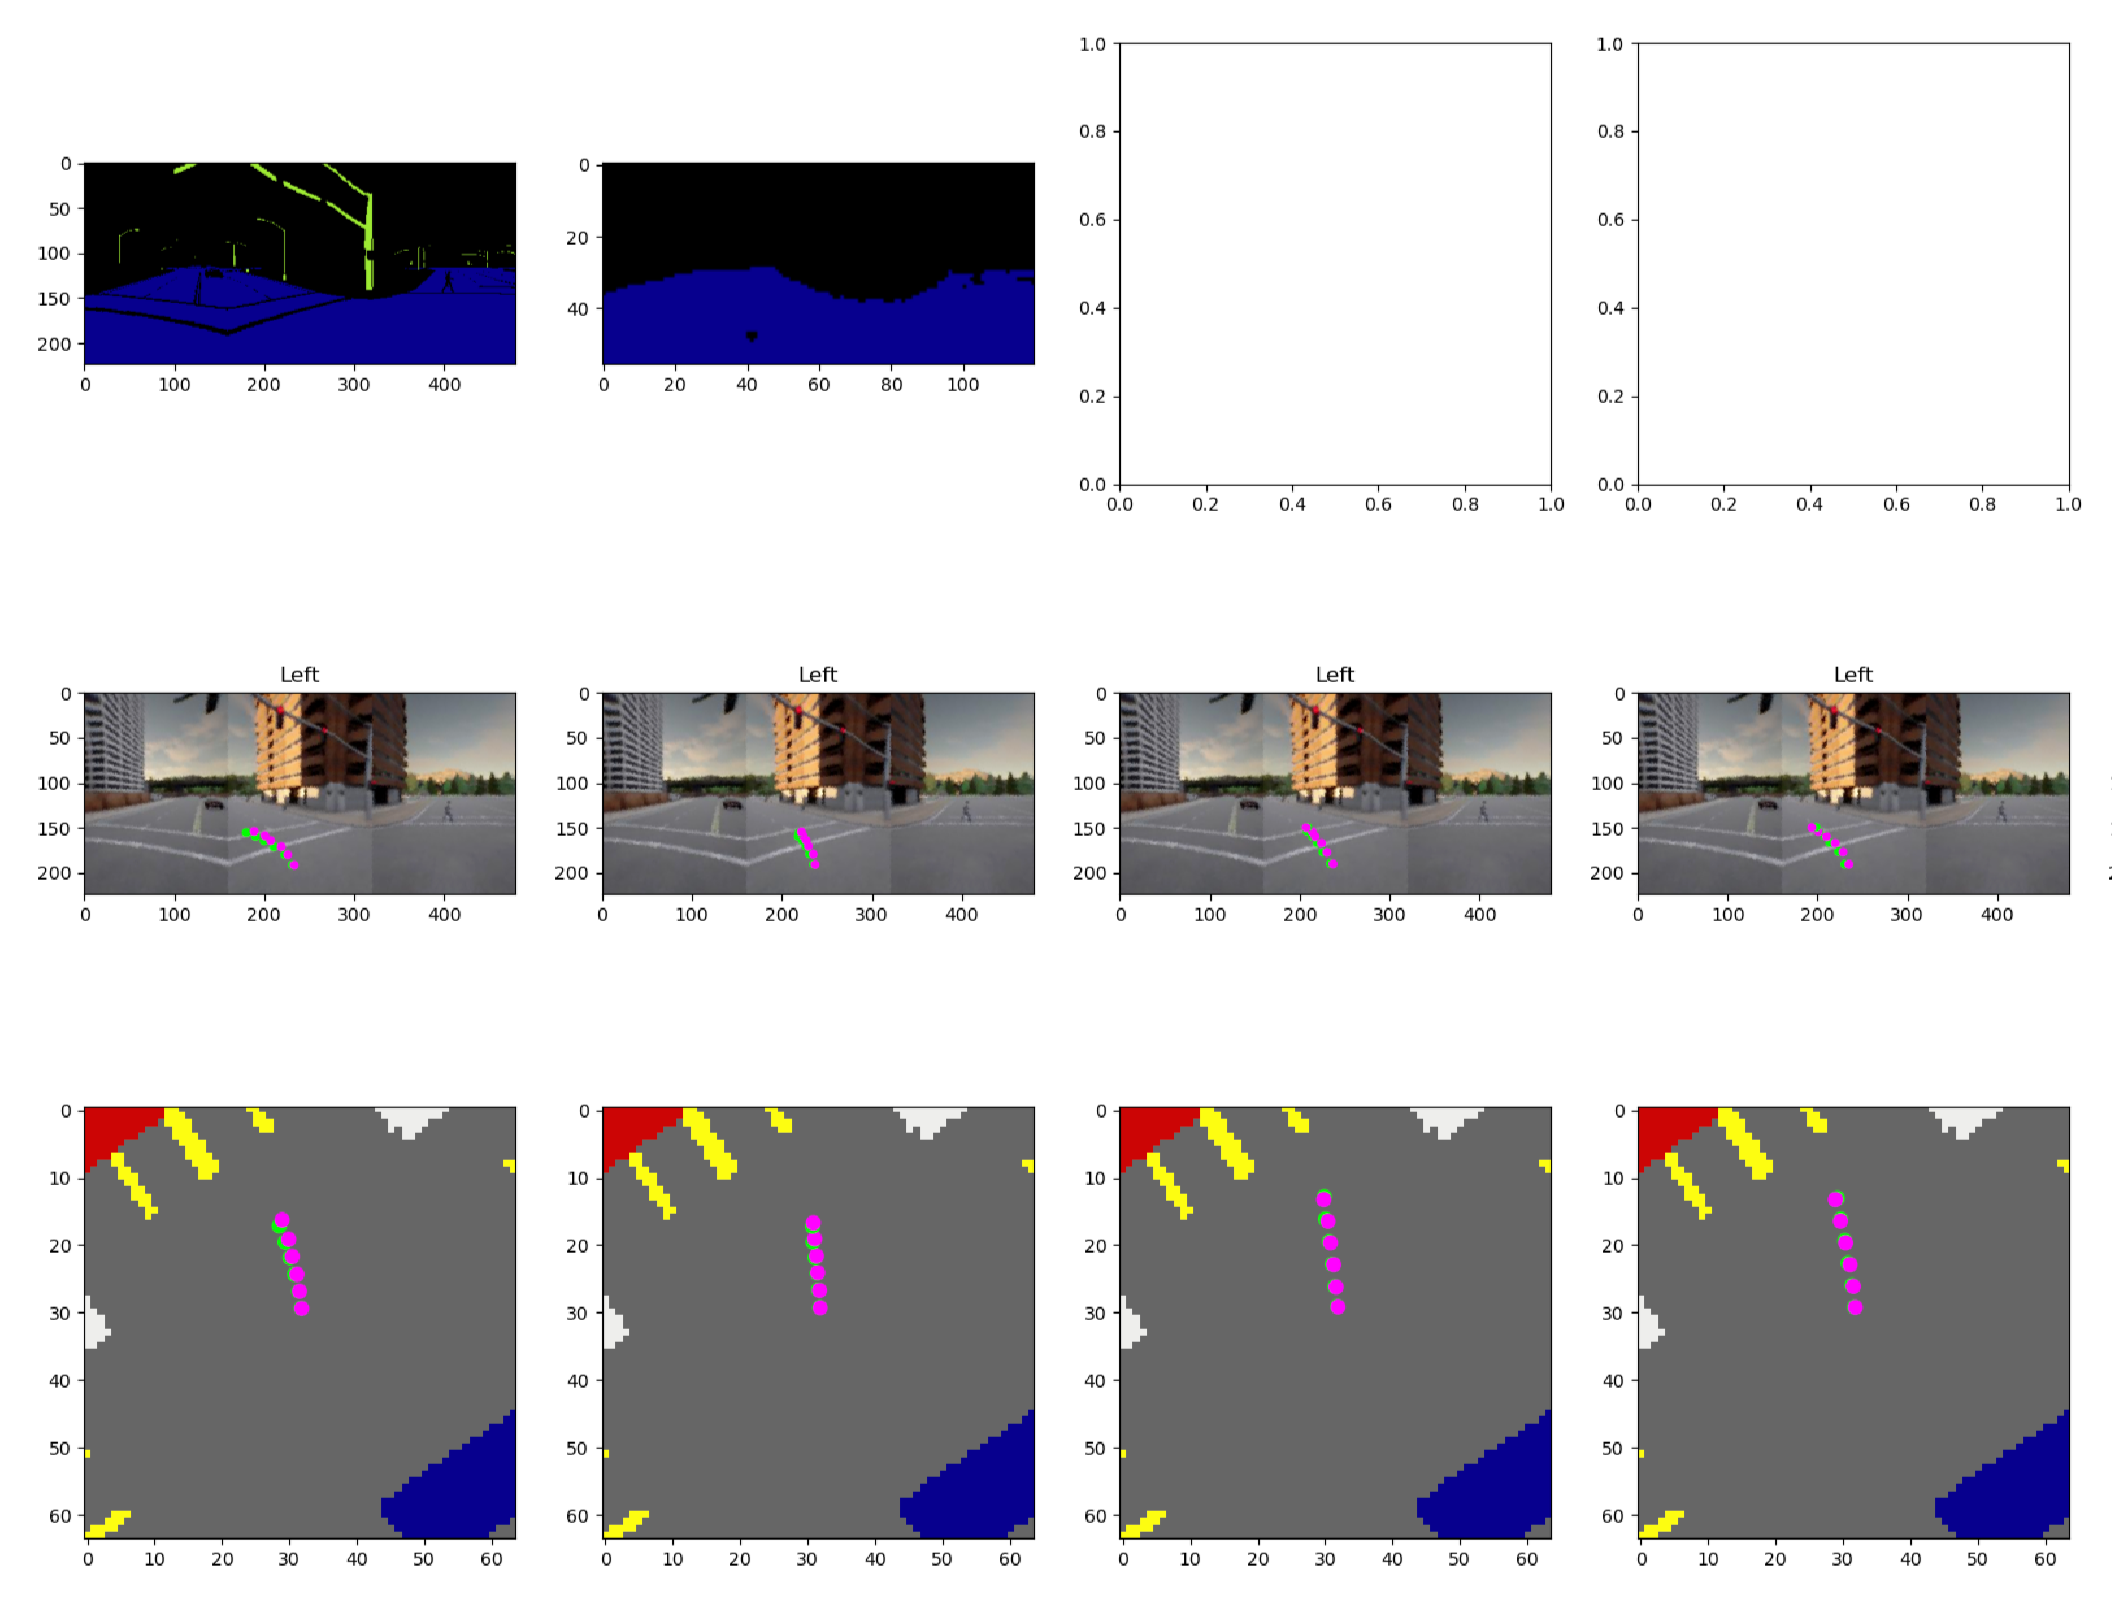
\includegraphics[width=0.8\textwidth] {bilder/northern_pyramid_683.png} 
  \caption{(green: ground truth, pink: predicted trajectory.) Later on, the model has learnt how to do the road segmentation, and can drive well.}
  %\label{fig:somesignal}
\end{figure}

% Section 4 ========================
\section {Results Evaluation and Comparison with Goals}
The author also provided their output for our reference. I think I got almost everything right. The model I trained outputs a reasonable trajectory, and it also learnt how to perceive the frontal camera images. Maybe it is a small pity that it has not learnt how to recognize the road lane, compared with the results the authors provided.
%[]
\begin{figure}[H]
  \centering
  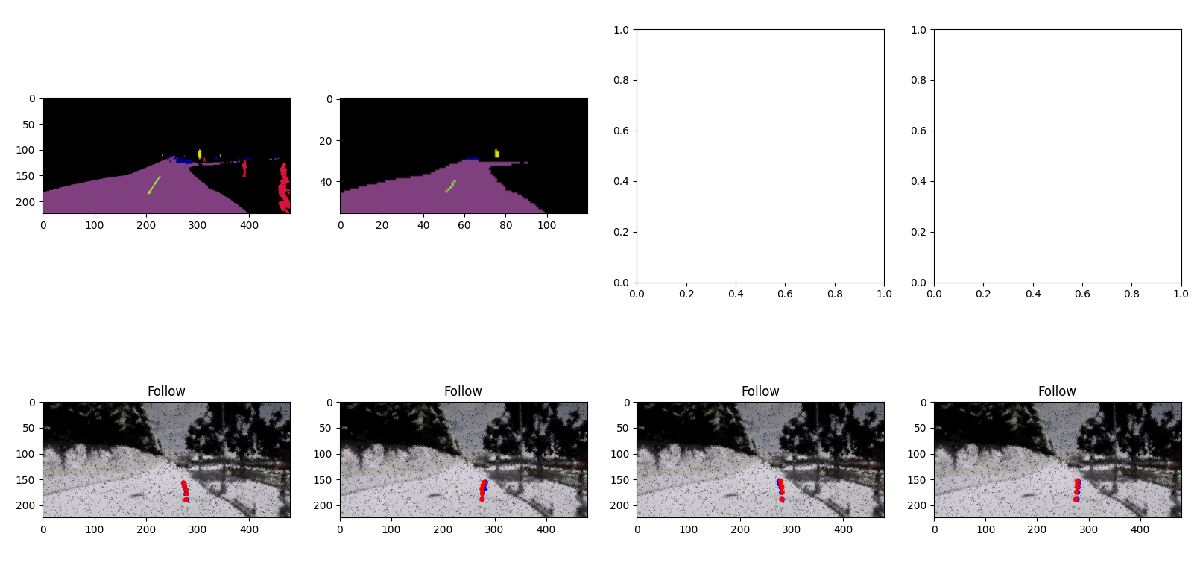
\includegraphics[width=0.8\textwidth] {bilder/lbc.jpg} 
  \caption{reference output from the authors}
  %\label{fig:somesignal}
\end{figure}

\noindent I did not really follow my initial plan in this internship, which was to implement a new model for motion planning. At the beginning, we were talking about only using the birds-eye-view map (not the frontal camera images) as the input, and implement a new idea. That was why I chose to use the privileged model from the LBC paper as the baseline. However, I was not really familiar with Python programming and deep learning practices. I had a lot to learn by just implementing a simple baseline. Even though I spent a lot of time discussing the theoretical part of the new idea with my supervisor, I still don’t know where to start if I’d like to implement it in a program. Hence, I chose to implement the sensorimotor and see how it performs.
\\

\noindent Now I have successfully trained both the privileged agent and the sensorimotor agent. The next step could be letting the agent run on the Carla simulator and see how it performs. However, at the moment I am more interested in how to optimize the training speed. I have observed a fluctuation in the time that my training episodes need. The first episode could take almost 12 hours, and I was using only one fourth of the whole given dataset. On the contrary, the later episodes sometimes only need 4 hours. Even if we exclude the first episode, since it is typical that the first one needs longer, I still see this fluctuation in the training time. Some episodes needed 4 to 5 hours, whereas the other ones needed up to 64 hours.
%[]

% Section 5 ========================
\section {Summary}
I have learnt a lot during this internship. Although I couldn’t make it to my supervisor’s expectation, I have already exceeded my own expectation. In the beginning, I didn’t think I could get anything working. But in the end, I got two models working.
\\

\noindent During this journey, I learnt a lot of the essential skills an engineer needs, which could not be taught in an university. I started to read papers just a few months ago because of this internship. I learnt how to work in a docker container on the server. I got more familiar with terminal commands. I started to use git because of this internship. I learnt how to use the debugger and how to manage virtual environments. I can program in python better and understand the code from other people faster now, compared with myself just two months ago. I gained real practices with deep learning and the framework PyTorch. I had a look into the research field, which was something I was always curious about.
\\

\noindent Last but not least, I would like to express my sincere thanks to my supervisor, Mr Matthes. No matter how many trivial questions I asked, he was always there and replied patiently. Additionally, I would like thank Mr Qiu and everyone else in the office who helped me out multiple times. I truly appreciate the support. 


\bibliography{other/citation}
\nocite{*}

\end{document}
